\section{Auswertung}
\label{sec:Auswertung}
Jegliche Fehlerrechnung wurde mit der python-Bibliothek uncertainties \cite{uncertainties} absolviert.
Trotz dessen sind die Formeln für die Unsicherheiten in den jeweiligen Abschnitten angegeben.
Allgemeine Rechnungen wurden mit der python-Bibliothek numpy \cite{numpy} automatisiert. 
Die graphischen Unterstützungen wurden mit Hilfe der python-Bibliothek matplotlib \cite{matplotlib} erstellt.\\
Die Bauteile der verwendeten Schaltung haben folgende Werte:
\begin{align*}
    L   & = \SI{16.78(9)} {\milli\henry}\\
    C   & = \SI{2.066(6)} {\nano\farad} \\
    R_1 & = \SI{67.2(2)}  {\ohm}        \\
    R_2 & = \SI{682(1)}   {\ohm} \; \text{.}
\end{align*}
\subsection{Bestimmung des Dämpfungswiderstandes}
In der Tabelle \ref{tab:voltage} ist die Spannung mit den dazugehörigen Zeiten aufgetragen.
\begin{table}
    \centering
    \caption{Gemessene Spannungsamplituden in Abhängigkeit von der Zeit}
    \label{tab:voltage}
    \begin{tabular} {S[table-format=4.1] S[table-format=2.2]}
        \toprule
        {$t \mathbin{/} \si{\micro\second}$} & {$U \mathbin{/} \si{\volt}$}  \\
    \midrule
    20      &   16.5\\
    60      &   14.0\\
    97      &   12.5\\
    135     &   10.5\\
    175     &   9\\
    212.5   &   8\\
    252.5   &   6.5\\
    290     &   5.75\\
    330     &   5.\\
    367.5   &   4.\\
    405     &   3.5\\
    442.5   &   3\\
    480.0   &   2.8\\
    520     &   2.4\\
    557.5   &   2\\
    595     &   1.8\\
    632.5   &   1.6\\
    670     &   1.4\\
    707.5   &   1.2\\
    745     &   1\\
    785     &   0.85\\
    822.5   &   0.75\\
    860     &   0.65\\
    897.5   &   0.55\\
    935     &   0.5\\
    972.5   &   0.4\\
    1010    &   0.35\\
    1047.5  &   0.3\\
    1085    &   0.26\\
    1125    &   0.24\\
    1162.5  &   0.2\\
    1200    &   0.16\\
    1237.5  &   0.14\\
    1275    &   0.12\\
    1312.5  &   0.08\\
    \bottomrule
\end{tabular}
\end{table}
\begin{figure}
    \centering
    \caption{Gemessene Spannungsamplituden mit Regression}
    \label{fig:voltage}
    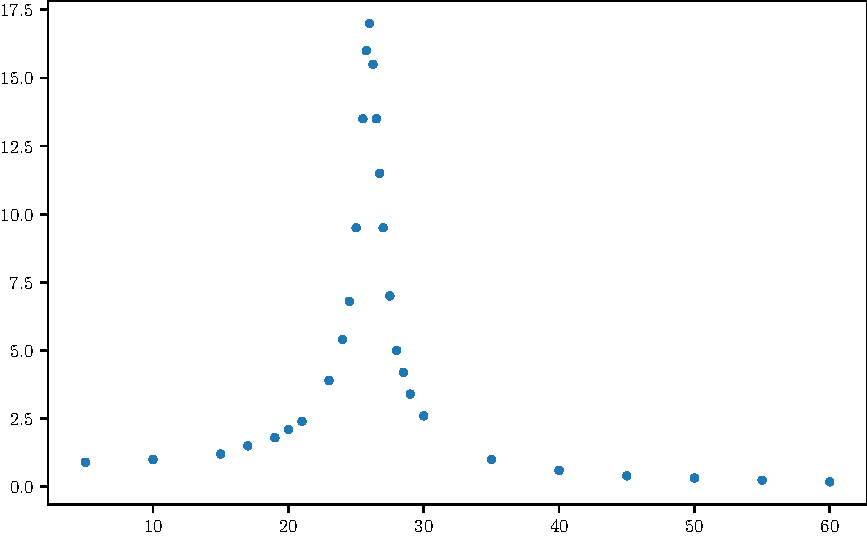
\includegraphics{build/voltage.pdf}
\end{figure}
Um den Dämpfungswiderstand zu bestimmen, ist es von Nöten eine Ausgleichsrechung mit dem $\symup{e}$-Term der Funktion
$REFERENZ$ durchzuführen.
Die Parameter der Regressionsfunktion
\begin{equation}
    U = U_0 \symup{e}^{-2\pi\mu t}
\end{equation}
lassen sich zu
\begin{align*}
    U_0 &= \SI{17.87(8)}{\volt}\\
    \mu &= \SI{622.51(92)}{\per\second}
\end{align*}
bestimmen.
Mit der Beziehung 
\begin{equation}
    R_\text{eff} = 4\pi\mu L 
\end{equation}
lässt sich der Dämpfungswiderstand R zu
\begin{equation*}
    R_\text{eff} = \SI{131.26(109)}{\ohm}
\end{equation*}
bestimmen.
Aus dem ebend berechneten Dämpfungswiderstand und der Gleichung $REFERENZ$ kann die Abklindauer zu 
\begin{equation*}
    T_\text{ex} = \SI{255.67(161)}{\micro\second}
\end{equation*}
errechnen.
Der Fehler für den Dämpfungswiderstand ergibt sich mittels Gaußscher Fehlerfortpflanzung zu 
\begin{equation}
    \symup{\Delta} R_\text{eff} = 4\pi \sqrt{L^2 \left( \symup{\Delta} \mu \right)^2  + \mu^2 \left( \symup{\Delta} L \right)^2} \; \text{}.
\end{equation}
Ebenfalls mittels Gaußscher Fehlerfortpflanzung ergibt sich der Fehler der Abklingzeit als
\begin{equation}
    \symup{\Delta} T_\text{ex} = \frac{2}{R_\text{eff}} \sqrt{\left( \symup{\Delta} L \right)^2 + \frac{L}{R_\text{eff}^2} \left( \symup{\Delta} R_\text{eff}  \right)^2 } \; \text{.}
\end{equation}
\subsection{Bestimmung des Dämpfungswiderstandes bei dem aperiodischen Grenzfall}
Während der Messung wurd ein Dämpfungswiderstand, bei dem der aperiodische Grenzfall eintritt, von
\begin{equation*}
    R_\text{ap} = \SI{4.4}{\kilo\ohm}
\end{equation*}
gemessen.
\subsection{}
\begin{figure}
    \centering
    \caption{Gemessene Spannungsamplituden mit den dazugehörigen Frequenzen}
    \label{fig:frequence}
    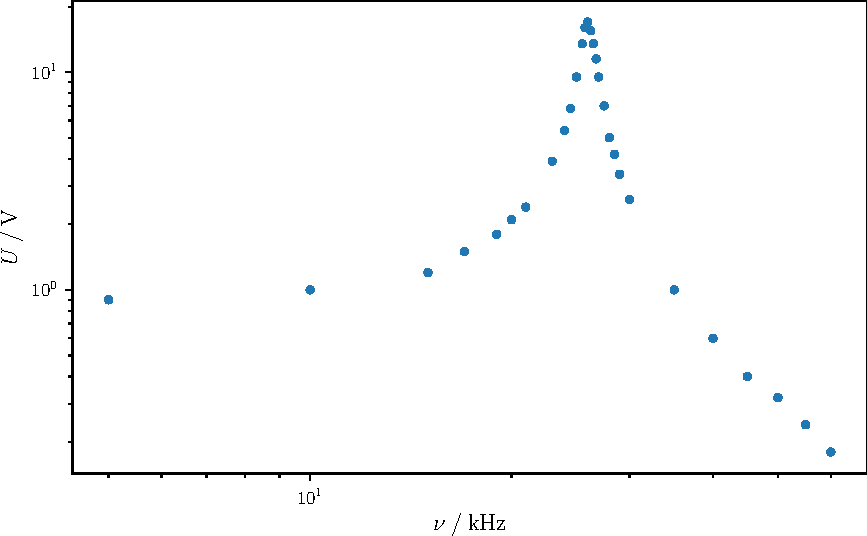
\includegraphics{build/frequence.pdf}
\end{figure}